\chapter{Design for X}
\label{ch7}

\paragraph{Where this fits.}
This chapter operates at Stage~3 (Development) of the Stage-Gate model.
Design-for-X decisions made here determine 70--80\,\% of manufacturing cost and
assembly quality before a single prototype board is soldered.
Catching a DFX violation at Stage~3 costs a design revision; the same violation
found at Stage~4 testing costs a board respin, a BOM change, and a schedule slip
that threatens Gate~4.

Chapter~6 selected the components that populate the architecture.
That fixed the bill of materials --- but not yet how the assembly, test procedure,
and reliability target will be designed into the hardware from the start.
This chapter supplies that discipline.

\begin{enumerate}
  \item Apply DFM principles to reduce unit cost for PCB and 3D-printed parts.
  \item Compute DFA assembly efficiency $\eta_A$ and identify parts that fail the
        keep/eliminate test.
  \item Design observability and controllability into a prototype using DFT principles:
        test points, debug ports, and built-in self-test.
  \item Connect the derating and lifecycle decisions from Chapter~6 to DFR design
        margin and thermal management.
\end{enumerate}

% ─────────────────────────────────────────────────────────────────────────────
\section{What DFX Means}
\label{sec:ch7-intro}
% ─────────────────────────────────────────────────────────────────────────────

\textbf{Design for X}\index{design for X} is the discipline of designing with the
downstream process in mind.
The ``X'' is a placeholder: it stands for Manufacturability (DFM), Assembly (DFA),
Test (DFT), or Reliability (DFR), and the four disciplines interact.

Figure~\ref{fig:ch7-dfx} shows the four domains and their relationship to prototype
design.

\begin{figure}[htbp]
  \centering
  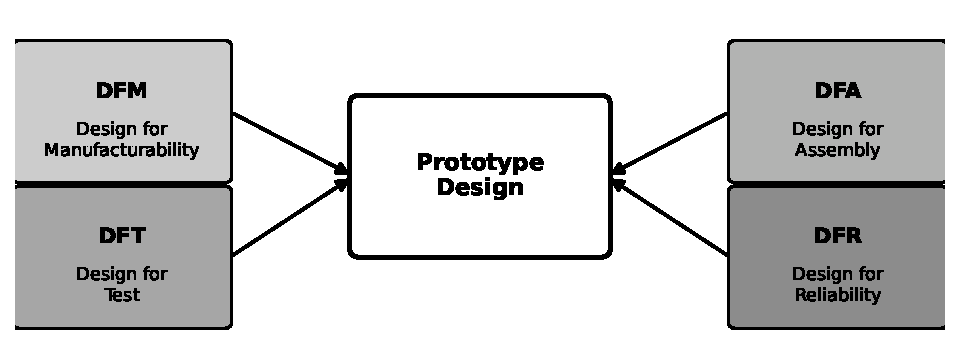
\includegraphics[width=0.85\textwidth]{images/fig_01_dfx_overview}
  \caption{The four DFX disciplines feed into every prototype design decision.
           Optimising one domain in isolation can degrade another; the goal is
           to resolve conflicts at Stage~3, before they become build failures.}
  \label{fig:ch7-dfx}
\end{figure}

A common misconception is that DFX is a checklist run at design-complete.
It is not.
DFX is a continuous design constraint: each time you choose a component, a trace
width, a fastener, or a PCB stack-up, you make a DFX decision.
If you make it consciously, using the principles in this chapter, you eliminate
whole categories of downstream failure.
If you make it by default, you pay for it at assembly, test, or field return.

% ─────────────────────────────────────────────────────────────────────────────
\section{Design for Manufacturability}
\label{sec:ch7-dfm}
% ─────────────────────────────────────────────────────────────────────────────

\textbf{Design for Manufacturability (DFM)}\index{design for manufacturability}
means choosing processes, tolerances, and geometries that standard equipment can
produce reliably at your target volume and cost.

\subsection{PCB DFM}
\label{sec:ch7-dfm-pcb}

The following rules apply to every prototype PCB submitted to a contract
manufacturer:

\begin{itemize}
  \item \textbf{Trace width and spacing.} Stay at or above the fabricator's
        minimum design rule.
        A 0.1~mm trace on a board specified for 0.15~mm minimum will be
        rejected or reflowed out of spec.
  \item \textbf{Via size.} Blind and buried vias cost extra; through-hole vias
        are standard.
        Choose via drill sizes that the fabricator's standard process supports.
  \item \textbf{Panelisation.} Design the board to panel at standard sizes so
        the fabricator can run multiple boards per panel without custom tooling.
  \item \textbf{Solder mask and silkscreen.} Solder mask openings must clear
        pad edges by the fabricator's specified clearance.
        Silkscreen must not overlap pads --- solder will not adhere through ink.
  \item \textbf{Component courtyard clearances.} Ensure no courtyard overlaps;
        the pick-and-place machine needs clear landing zones for each nozzle.
\end{itemize}

\subsection{3D-Print DFM}
\label{sec:ch7-dfm-3dp}

The running example uses a 3D-printed housing.
FDM (fused deposition modelling) imposes its own DFM rules:

\begin{itemize}
  \item \textbf{Minimum wall thickness.} FDM walls thinner than 1.2~mm (two
        perimeters at 0.4~mm nozzle) are weak and prone to delamination.
  \item \textbf{Overhang angle.} Overhangs beyond 45\textdegree{} require
        support material, which must be removed and damages fine features.
        Design with 45\textdegree{} chamfers instead of 60\textdegree{} ledges.
  \item \textbf{Part orientation.} Orient the part so that the functional
        mating surfaces (connector openings, PCB standoffs) are printed in the
        XY plane, not the Z direction, where layer adhesion is weaker.
  \item \textbf{Support-free internal channels.} Route cable channels as
        tear-drop cross-sections rather than round bores; they print without
        support and are stronger.
\end{itemize}

\paragraph{In Practice.}
A 3D-printed housing for the running example was designed with 60\textdegree{}
overhangs on the internal PCB shelf.
Support material filled the shelf cavity; removing it with pliers cracked the
shelf on two of six printed units.
Redesigning to a 45\textdegree{} chamfer eliminated the support requirement
entirely, and all subsequent units printed clean.

% ─────────────────────────────────────────────────────────────────────────────
\section{Design for Assembly}
\label{sec:ch7-dfa}
% ─────────────────────────────────────────────────────────────────────────────

\textbf{Design for Assembly (DFA)}\index{design for assembly} minimises the
number of parts and assembly operations, reducing labour cost and assembly
error rate.

\subsection{The Boothroyd--Dewhurst Criterion}
\label{sec:ch7-dfa-bd}

The \textbf{Boothroyd--Dewhurst keep/eliminate test}\index{Boothroyd--Dewhurst
criterion} asks three questions for each part:

\begin{enumerate}
  \item Does the part move relative to all other parts during operation?
  \item Must the part be made of a different material from adjacent parts?
  \item Must the part be separate to allow assembly or disassembly?
\end{enumerate}

A part that answers \emph{no} to all three questions is a candidate for
elimination --- it can be integrated into an adjacent part.
$N_{\min}$ is the count of parts that answer \emph{yes} to at least one question.

\subsection{Assembly Efficiency}
\label{sec:ch7-dfa-eta}

\textbf{Assembly efficiency}\index{assembly efficiency} $\eta_A$ measures how
close a design is to the theoretical minimum:
%
\begin{equation}
  \label{eq:ch7-dfa}
  \eta_A = \frac{N_{\min} \cdot t_{\text{ideal}}}{t_{\text{actual}}}
\end{equation}
%
where $t_{\text{ideal}} = 3$~s is the Boothroyd--Dewhurst standard ideal assembly
time per part, and $t_{\text{actual}}$ is the measured total assembly time in
seconds.
A higher $\eta_A$ means the design is closer to the minimum.
Typical values for a first-pass design are 5--15\,\%; well-optimised assemblies
reach 40--60\,\%.

The cost saving from a DFA redesign is:
%
\begin{equation}
  \label{eq:ch7-dfm-cost}
  \Delta C \approx \Delta N_{\text{parts}} \cdot \bar{c}_{\text{part}}
               + \Delta N_{\text{ops}} \cdot \bar{c}_{\text{op}}
\end{equation}
%
where $\bar{c}_{\text{part}}$ is the average part cost saved per eliminated part
and $\bar{c}_{\text{op}}$ is the average cost per assembly operation second
(typically \$0.08--\$0.15/s at contract assembly rates in CAD).

% ─────────────────────────────────────────────────────────────────────────────
\section{Design for Test}
\label{sec:ch7-dft}
% ─────────────────────────────────────────────────────────────────────────────

\textbf{Design for Test (DFT)}\index{design for test} builds observability and
controllability into the hardware at design time.
\textbf{Observability}\index{observability} means you can measure a signal's
actual value.
\textbf{Controllability}\index{controllability} means you can force a signal to
a known state to isolate a fault.

Figure~\ref{fig:ch7-dft} shows the three DFT features designed into the
running-example MCU board: test points, a UART debug header, and an SWD/JTAG
programming header.

\begin{figure}[htbp]
  \centering
  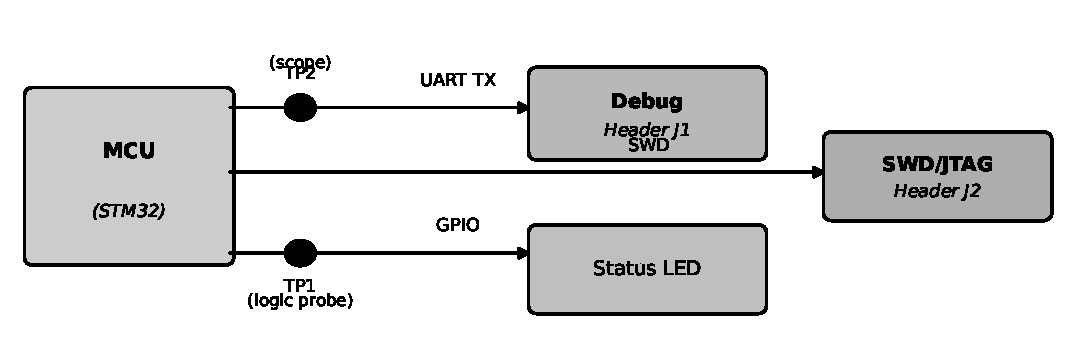
\includegraphics[width=0.85\textwidth]{images/fig_03_dft_testpoints}
  \caption{DFT features on the running-example MCU board: test points TP1 and TP2
           accessible by a logic probe and scope respectively; a UART debug header
           (J1) for firmware printf output; an SWD/JTAG header (J2) for breakpoint
           debugging and firmware flashing.}
  \label{fig:ch7-dft}
\end{figure}

\subsection{Test Points}
\label{sec:ch7-dft-tp}

\textbf{Test points}\index{test point} are labelled, exposed pads or through-hole
vias placed on every signal that a technician might need to probe.
Minimum rules:
\begin{itemize}
  \item One test point per power rail, placed between the regulator output and
        the first load capacitor.
  \item One test point on every high-frequency or safety-critical signal.
  \item Test points must be at least 2.54~mm from any component body to allow
        a standard probe tip to land.
\end{itemize}

\subsection{Debug Ports and BIST}
\label{sec:ch7-dft-debug}

A \textbf{UART debug port}\index{UART debug port} connected to a header allows
the firmware to stream printf output during development without stopping
execution.
This exposes firmware state non-intrusively --- the single most valuable DFT
feature for firmware-heavy prototypes.

\textbf{Built-in self-test (BIST)}\index{built-in self-test} is firmware that
runs a self-check sequence at power-on, toggles each output GPIO, reads back
each ADC rail, and reports pass/fail over the debug port before the main
application loop starts.
BIST catches bring-up faults in under 30~seconds.

\subsection{Defect Coverage}
\label{sec:ch7-dft-dpmo}

Once test procedures are running, track defect density with
\textbf{DPMO}\index{DPMO} (defects per million opportunities):
%
\begin{equation}
  \label{eq:ch7-dpmo}
  \mathrm{DPMO} = \frac{D}{N \cdot O} \times 10^{6}
\end{equation}
%
where $D$ is the number of defects observed, $N$ is the number of units tested,
and $O$ is the number of test opportunities per unit.
Adding more test points increases $O$, which lowers DPMO for the same physical
defect count --- this is the quantitative argument for investing in DFT.

\paragraph{In Practice.}
An early prototype of the running-example sorter board had no test points and no
UART debug port.
When the sort classifier produced incorrect results during bring-up, the
validation team spent three days probing unmarked pads with a clip lead to
distinguish a firmware logic error from a hardware signal-integrity problem.
A UART debug port would have printed the classifier output at each step and
isolated the fault in under 20~minutes.
The three days were not recoverable from the project schedule.

% ─────────────────────────────────────────────────────────────────────────────
\section{Design for Reliability}
\label{sec:ch7-dfr}
% ─────────────────────────────────────────────────────────────────────────────

\textbf{Design for Reliability (DFR)}\index{design for reliability} translates
the FMEA risk register from Chapter~4 and the derating margins from Chapter~6
into concrete design choices.

\subsection{Derating and FMEA Margin}
\label{sec:ch7-dfr-margin}

The derating factor $D_f$ from Chapter~6 is a DFR parameter: a component
operating at $D_f = 0.70$ has significantly longer expected life than one at
$D_f = 0.90$.
When the FMEA assigns Severity~$S \geq 8$ to a failure mode, the DFR response
is to increase the design margin --- lower $D_f$, specify a higher-rated part,
or add protective circuitry.

\subsection{Redundancy}
\label{sec:ch7-dfr-redundancy}

For failure modes that are both high-severity and high-occurrence (RPN $> 80$
from Chapter~4), \textbf{redundancy}\index{redundancy} may be justified:
two components in parallel, where either one suffices, lower the effective
failure rate.
Use Chapter~6's parallel-reliability equation to quantify the improvement before
committing board area.

\subsection{Thermal Management}
\label{sec:ch7-dfr-thermal}

Every power-dissipating component has a maximum junction temperature $T_{j,\max}$.
The thermal budget is:
\[
  T_j = T_{\text{ambient}} + P_D \cdot \theta_{JA}
\]
where $P_D$ is power dissipation and $\theta_{JA}$ is junction-to-ambient
thermal resistance from the datasheet.
Verify $T_j < T_{j,\max}$ at maximum operating ambient temperature before
finalising component placement; hotspot components may need copper pours,
thermal vias, or forced airflow.

% ─────────────────────────────────────────────────────────────────────────────
\section{DFX Trade-offs in Practice}
\label{sec:ch7-tradeoffs}
% ─────────────────────────────────────────────────────────────────────────────

The four disciplines interact and sometimes conflict.
A DFM optimisation (reducing layer count to save fabrication cost) may eliminate
the reference plane needed for signal integrity (a DFR regression).
A DFA optimisation (integrating two parts into one moulded piece) may block the
disassembly access required for test (a DFT regression).

The resolution principle is: \emph{optimise for the dominant cost driver at your
production volume}.

\begin{itemize}
  \item At \textbf{prototype volume} (1--10 units): labour time dominates.
        Prioritise DFT --- instrument every signal, use every debug port.
        DFM is secondary; a few extra fabrication days matter less than a
        three-day firmware debug.
  \item At \textbf{low-volume production} (100--1000 units): assembly cost
        dominates.
        Prioritise DFA --- eliminate parts, standardise fasteners, design for
        one-directional insertion.
  \item At \textbf{high volume} (10\,000+): material cost dominates.
        Prioritise DFM --- optimise BOM cost, panel efficiency, and process yield.
\end{itemize}

\paragraph{Common Pitfalls.}
DFX applied as a post-design review checklist rather than a live design
constraint will always find violations too late to fix cheaply.
Every design decision from component selection onward is a DFX decision; treat
it that way.

\paragraph{Common Pitfalls.}
Adding test points ``if there is room'' is not DFT.
Test points designed in as required features, with reserved courtyard space and
silkscreen labels, are DFT.
Three strategically placed test points found a PCB fabrication defect in the
running example during bring-up; three test points added as afterthoughts on the
same board revealed nothing because they landed on signals that were already
observable with a multimeter.

% ─────────────────────────────────────────────────────────────────────────────
\section{Worked Example}
\label{sec:ch7-worked}
% ─────────────────────────────────────────────────────────────────────────────

The running-example sorter board has an eight-part PCB subassembly.
Applying the Boothroyd--Dewhurst test, three parts must be kept ($N_{\min} = 3$):
the MCU (different material and function), the motor-driver IC (different
material and function), and the connector housing (must be separate for mating
access).
The remaining five parts --- three identical M2 standoffs, one wire-tie anchor,
and one redundant power-rail capacitor --- answer \emph{no} to all three
questions and are candidates for elimination.

\subsection*{Part A --- Assembly Efficiency}

Before redesign: $N_{\text{parts}} = 8$, $t_{\text{actual}} = 120$~s.

Using Equation~\ref{eq:ch7-dfa}:
\[
  \eta_A = \frac{N_{\min} \cdot t_{\text{ideal}}}{t_{\text{actual}}}
         = \frac{3 \times 3}{120}
         = \frac{9}{120}
         = 0.075 \quad (7.5\,\%)
\]

Two parts are eliminated in the redesign (the three standoffs become integrated
PCB snap features; the wire-tie anchor is removed by routing the cable through a
slot moulded into the housing).
The redesign reduces $t_{\text{actual}}$ to 80~s.

\[
  \eta_A' = \frac{3 \times 3}{80} = \frac{9}{80} = 0.1125 \quad (11.25\,\%)
\]

Figure~\ref{fig:ch7-dfa} shows the before/after comparison.

\begin{figure}[htbp]
  \centering
  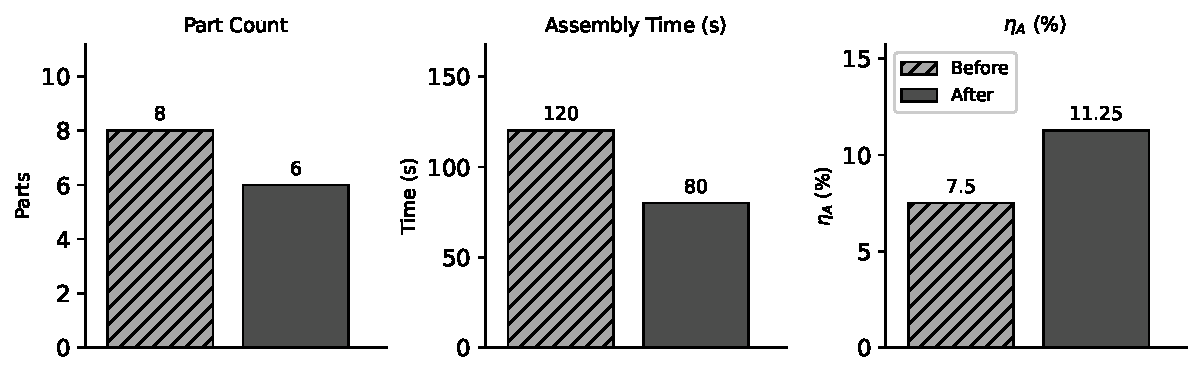
\includegraphics[width=0.85\textwidth]{images/fig_02_dfa_parts}
  \caption{Part count, assembly time, and $\eta_A$ before and after
           the DFA redesign. Eliminating two parts reduces assembly time by
           33\,\% and raises $\eta_A$ from 7.5\,\% to 11.25\,\%.}
  \label{fig:ch7-dfa}
\end{figure}

Using Equation~\ref{eq:ch7-dfm-cost} with $\bar{c}_{\text{op}} = \$0.10$/s and
a production run of 500 units:
\[
  \Delta C = (120 - 80)\,\text{s} \times \$0.10/\text{s} \times 500
           = 40 \times \$0.10 \times 500
           = \$2{,}000 \text{ CAD}
\]

\subsection*{Part B --- Defect Coverage (DPMO)}

A test run of 100 units of the sorter PCB subassembly produces 3 defects.
Each unit has $O = 12$ test opportunities (12 explicitly designed test points).

Using Equation~\ref{eq:ch7-dpmo}:
\[
  \mathrm{DPMO} = \frac{D}{N \cdot O} \times 10^{6}
               = \frac{3}{100 \times 12} \times 10^{6}
               = \frac{3}{1200} \times 10^{6}
               = 2{,}500 \text{ DPMO}
\]

At this rate, a production run of 10\,000 units would yield:
\[
  10{,}000 \times 12 \times \frac{2{,}500}{10^{6}} = 300 \text{ defective opportunities}
\]
Interpreted: 300 test points across all units will fail; each failure triggers
a rework or rejection.

% ─────────────────────────────────────────────────────────────────────────────
\subsection*{Try It Yourself}
% ─────────────────────────────────────────────────────────────────────────────

A sensor breakout board subassembly has 6 parts, $t_{\text{actual}} = 90$~s, and
$N_{\min} = 2$.
The team identifies one candidate for elimination (a redundant tie-point bracket),
reducing $t_{\text{actual}}$ to 65~s.
A test run of 50 units reveals 2 defects; each unit has 8 test opportunities.

\begin{enumerate}
  \item[(a)] Compute $\eta_A$ before the elimination using
             Equation~\ref{eq:ch7-dfa}.
  \item[(b)] Compute $\eta_A$ after the elimination.
  \item[(c)] Compute the assembly cost saving per unit at 200 units using
             $\bar{c}_{\text{op}} = \$0.10$/s (Equation~\ref{eq:ch7-dfm-cost}).
  \item[(d)] Compute the DPMO using Equation~\ref{eq:ch7-dpmo}.
\end{enumerate}

\noindent(No answer key provided.)

% ─────────────────────────────────────────────────────────────────────────────
\section*{Review Questions}
% ─────────────────────────────────────────────────────────────────────────────

\begin{enumerate}

  \item \textbf{(Conceptual)} State the four DFX disciplines covered in this
  chapter.
  For each, give one specific design decision from the running-example sorter
  prototype that falls within that discipline.

  \item \textbf{(Conceptual)} Explain the Boothroyd--Dewhurst three-question
  keep/eliminate test.
  Give one example of a component that passes all three criteria (must be kept)
  and one that fails all three (candidate for elimination) from the running
  example.

  \item \textbf{(Applied --- calculation)} A subassembly has 10 parts and
  $t_{\text{actual}} = 150$~s.
  The Boothroyd--Dewhurst test identifies $N_{\min} = 4$.
  \begin{enumerate}
    \item[(a)] Compute $\eta_A$ using Equation~\ref{eq:ch7-dfa}.
    \item[(b)] A redesign eliminates 3 parts and reduces $t_{\text{actual}}$ to
               100~s.
               Compute the new $\eta_A$.
    \item[(c)] Compute the assembly cost saving per unit at 300 units, using
               $\bar{c}_{\text{op}} = \$0.12$/s.
  \end{enumerate}

  \item \textbf{(Applied --- multi-step)} A production run of 200 units yields
  5 defects, with $O = 15$ test opportunities per unit.
  \begin{enumerate}
    \item[(a)] Compute DPMO using Equation~\ref{eq:ch7-dpmo}.
    \item[(b)] At this rate, how many defects are expected in a run of
               50\,000 units?
    \item[(c)] The team adds 3 additional test points per unit, raising $O$
               from 15 to 18.
               The defect count stays at 5 per 200 units.
               Recompute DPMO and explain in one sentence why DPMO decreased
               even though the physical defect count did not change.
  \end{enumerate}

  \item \textbf{(Conceptual)} Explain why DFM and DFA can conflict.
  Give one example where reducing material cost (DFM) increases assembly time
  (DFA regression).
  State how to decide which discipline to prioritise at prototype volume versus
  production volume.

\end{enumerate}

% ─────────────────────────────────────────────────────────────────────────────
\section*{Portfolio Entry}
\addcontentsline{toc}{section}{Portfolio Entry}
\label{sec:ch7-artifact}
% ─────────────────────────────────────────────────────────────────────────────

Your DFX review checklist for the prototype:

\begin{enumerate}
  \item \textbf{DFM} --- three PCB or mechanical decisions that use standard
        processes: trace width and via size within fabricator rules; 3D-print
        features within 45\textdegree{} overhang limit; panel size within
        standard sheet.
  \item \textbf{DFA} --- $\eta_A$ computed for the most complex subassembly;
        one elimination candidate identified and either eliminated or logged with
        justification for retention.
  \item \textbf{DFT} --- three observability features explicitly designed in:
        test-point locations and labelled signals; UART debug port with header
        and silkscreen designation; BIST firmware routine described.
  \item \textbf{DFR} --- derating margin from Chapter~6 confirmed against the
        FMEA Severity ratings from Chapter~4; any $D_f > 0.80$ entry resolved or
        logged as a risk item for Gate~3.
\end{enumerate}

% ─────────────────────────────────────────────────────────────────────────────
\section*{Chapter Summary}
\addcontentsline{toc}{section}{Chapter Summary}
\label{sec:ch7-summary}
% ─────────────────────────────────────────────────────────────────────────────

Four disciplines now constrain your prototype design before the first component
is soldered.
DFM aligns your PCB layout and 3D geometry with what standard processes can
produce reliably.
DFA uses the Boothroyd--Dewhurst criterion and $\eta_A$ (Equation~\ref{eq:ch7-dfa})
to quantify and reduce assembly labour.
DFT instruments every critical signal with test points, debug ports, and BIST so
that bring-up faults are found in minutes rather than days.
DFR translates FMEA severity ratings and derating margins into design choices
that protect reliability before the hardware is built.

The DFX checklist you produced is a concrete Stage~3 deliverable.
Gate~3 reviewers will look for evidence that cost, assembly, and reliability
were designed in, not discovered during validation.

Chapter~7 disciplined the design process.
Chapter~8 now introduces AI tools that can accelerate design work --- and
explains how to use them without compromising the engineer's accountability
for every output.

